\documentclass[tikz,border=0pt]{standalone}
\usepackage[T1]{fontenc}
\usepackage{lmodern}
\usetikzlibrary{arrows.meta}
\renewcommand{\familydefault}{\sfdefault}
\begin{document}
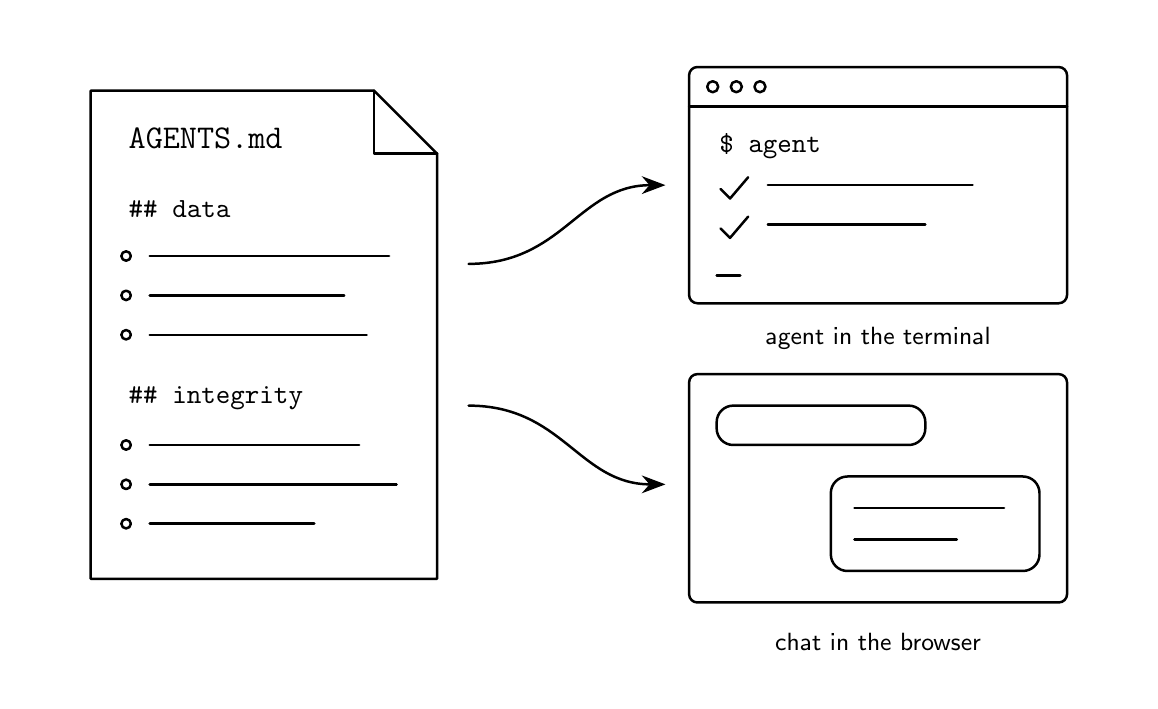
\begin{tikzpicture}[line width=0.9pt, line cap=round, line join=round, font=\sffamily]
  % 16:9 frame (invisible, fixes the aspect ratio)
  \path (1.2,0.1) rectangle (15.2,8.4);

  % Instruction file with folded corner
  \draw (2,1.4) -- (2,7.6) -- (5.6,7.6) -- (6.4,6.8) -- (6.4,1.4) -- cycle;
  \draw (5.6,7.6) -- (5.6,6.8) -- (6.4,6.8);
  \node[anchor=west, font=\ttfamily\large] at (2.35,7.0) {AGENTS.md};
  \node[anchor=west, font=\ttfamily] at (2.35,6.1) {\#\# data};
  \foreach \y/\l in {5.5/3.2, 5.0/2.6, 4.5/2.9} {
    \draw (2.45,\y) circle (0.06);
    \draw (2.75,\y) -- (2.75+\l*0.95,\y);
  }
  \node[anchor=west, font=\ttfamily] at (2.35,3.7) {\#\# integrity};
  \foreach \y/\l in {3.1/2.8, 2.6/3.3, 2.1/2.2} {
    \draw (2.45,\y) circle (0.06);
    \draw (2.75,\y) -- (2.75+\l*0.95,\y);
  }

  % Arrows
  \draw[-{Stealth[length=3mm]}] (6.8,5.4) .. controls (8.0,5.4) and (8.2,6.4) .. (9.3,6.4);
  \draw[-{Stealth[length=3mm]}] (6.8,3.6) .. controls (8.0,3.6) and (8.2,2.6) .. (9.3,2.6);

  % Terminal window
  \draw[rounded corners=3pt] (9.6,4.9) rectangle (14.4,7.9);
  \draw (9.6,7.4) -- (14.4,7.4);
  \foreach \x in {9.9,10.2,10.5} \draw (\x,7.65) circle (0.07);
  \node[anchor=west, font=\ttfamily] at (9.85,6.9) {\$ agent};
  \draw (10.0,6.35) -- (10.12,6.23) -- (10.35,6.5);
  \draw (10.6,6.4) -- (13.2,6.4);
  \draw (10.0,5.85) -- (10.12,5.73) -- (10.35,6.0);
  \draw (10.6,5.9) -- (12.6,5.9);
  \draw (9.95,5.25) -- (10.25,5.25);
  \node[font=\small] at (12,4.45) {agent in the terminal};

  % Chat window
  \draw[rounded corners=3pt] (9.6,1.1) rectangle (14.4,4.0);
  \draw[rounded corners=6pt] (9.95,3.1) rectangle (12.6,3.6);
  \draw[rounded corners=6pt] (11.4,1.5) rectangle (14.05,2.7);
  \draw (11.7,2.3) -- (13.6,2.3);
  \draw (11.7,1.9) -- (13.0,1.9);
  \node[font=\small] at (12,0.6) {chat in the browser};
\end{tikzpicture}
\end{document}
